% \documentclass{standalone}

% \input{../tikz_header}

% \begin{document}



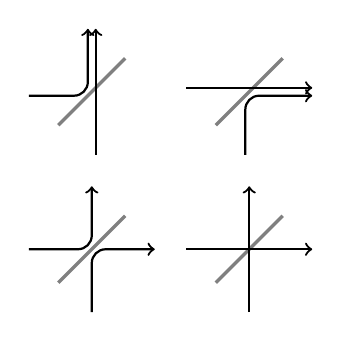
\begin{tikzpicture}%[font=\footnotesize]
%\useasboundingbox (0,0) rectangle (5,5);
%\draw (0,0) rectangle (5,5);

\pgfmathsetmacro{\x}{0.05}
\pgfmathsetmacro{\L}{0.8}

\begin{scope}% bottom left
\draw[very thick, gray] (45:0.6) -- (45:-0.6);

\draw [thick, rounded corners=5pt, ->] (-\L, 0)  -- (0,0) -- (0, \L);
\draw [thick, rounded corners=5pt, ->] (0, -\L)  -- (0,0) -- (\L, 0);
\end{scope}

\begin{scope}[xshift=20mm] % bottom right
    \draw[very thick, gray] (45:0.6) -- (45:-0.6);
    
    \draw [thick, rounded corners=5pt, ->] (-\L, 0)   -- (\L, 0);
    \draw [thick, rounded corners=5pt, ->] (0, -\L)  -- (0, \L);
\end{scope}

\begin{scope}[yshift=20mm]  % top left
    \draw[very thick, gray] (45:0.6) -- (45:-0.6);
    
    \draw [thick, rounded corners=5pt, ->] (-\L, -\x)  -- (-\x, -\x) -- (-\x, \L);
    \draw [thick, rounded corners=5pt, ->] (\x, -\L)   -- (\x, \L);
\end{scope}

\begin{scope}[xshift=20mm, yshift=20mm] % top right
    \draw[very thick, gray] (45:0.6) -- (45:-0.6);
    
    \draw [thick, rounded corners=5pt, ->] (-\L, \x)   -- (\L,  \x);
    \draw [thick, rounded corners=5pt, ->] (-\x, -\L)  -- (-\x, -\x) -- (\L, -\x);
\end{scope}

\end{tikzpicture}


%\end{document}